% Options for packages loaded elsewhere
\PassOptionsToPackage{unicode}{hyperref}
\PassOptionsToPackage{hyphens}{url}
%
\documentclass[
  twocolumn]{article}
\usepackage{amsmath,amssymb}
\usepackage{lmodern}
\usepackage{ifxetex,ifluatex}
\ifnum 0\ifxetex 1\fi\ifluatex 1\fi=0 % if pdftex
  \usepackage[T1]{fontenc}
  \usepackage[utf8]{inputenc}
  \usepackage{textcomp} % provide euro and other symbols
\else % if luatex or xetex
  \usepackage{unicode-math}
  \defaultfontfeatures{Scale=MatchLowercase}
  \defaultfontfeatures[\rmfamily]{Ligatures=TeX,Scale=1}
\fi
% Use upquote if available, for straight quotes in verbatim environments
\IfFileExists{upquote.sty}{\usepackage{upquote}}{}
\IfFileExists{microtype.sty}{% use microtype if available
  \usepackage[]{microtype}
  \UseMicrotypeSet[protrusion]{basicmath} % disable protrusion for tt fonts
}{}
\makeatletter
\@ifundefined{KOMAClassName}{% if non-KOMA class
  \IfFileExists{parskip.sty}{%
    \usepackage{parskip}
  }{% else
    \setlength{\parindent}{0pt}
    \setlength{\parskip}{6pt plus 2pt minus 1pt}}
}{% if KOMA class
  \KOMAoptions{parskip=half}}
\makeatother
\usepackage{xcolor}
\IfFileExists{xurl.sty}{\usepackage{xurl}}{} % add URL line breaks if available
\IfFileExists{bookmark.sty}{\usepackage{bookmark}}{\usepackage{hyperref}}
\hypersetup{
  pdftitle={Red Wood Data Analysis Report},
  pdfauthor={Andrew Amore, Dylan (Shi-Ting) Lu},
  hidelinks,
  pdfcreator={LaTeX via pandoc}}
\urlstyle{same} % disable monospaced font for URLs
\usepackage[margin=1in]{geometry}
\usepackage{longtable,booktabs,array}
\usepackage{calc} % for calculating minipage widths
% Correct order of tables after \paragraph or \subparagraph
\usepackage{etoolbox}
\makeatletter
\patchcmd\longtable{\par}{\if@noskipsec\mbox{}\fi\par}{}{}
\makeatother
% Allow footnotes in longtable head/foot
\IfFileExists{footnotehyper.sty}{\usepackage{footnotehyper}}{\usepackage{footnote}}
\makesavenoteenv{longtable}
\usepackage{graphicx}
\makeatletter
\def\maxwidth{\ifdim\Gin@nat@width>\linewidth\linewidth\else\Gin@nat@width\fi}
\def\maxheight{\ifdim\Gin@nat@height>\textheight\textheight\else\Gin@nat@height\fi}
\makeatother
% Scale images if necessary, so that they will not overflow the page
% margins by default, and it is still possible to overwrite the defaults
% using explicit options in \includegraphics[width, height, ...]{}
\setkeys{Gin}{width=\maxwidth,height=\maxheight,keepaspectratio}
% Set default figure placement to htbp
\makeatletter
\def\fps@figure{htbp}
\makeatother
\setlength{\emergencystretch}{3em} % prevent overfull lines
\providecommand{\tightlist}{%
  \setlength{\itemsep}{0pt}\setlength{\parskip}{0pt}}
\setcounter{secnumdepth}{-\maxdimen} % remove section numbering
\usepackage{titlesec}
\titlespacing{\section}{0pt}{12pt plus 2pt minus 1pt}{0pt plus 1pt minus 1pt}
\titlespacing{\subsection}{0pt}{12pt plus 2pt minus 1pt}{0pt plus 1pt minus 1pt}
\titlespacing{\subsubsection}{0pt}{12pt plus 2pt minus 1pt}{0pt plus 1pt minus 1pt}
\ifluatex
  \usepackage{selnolig}  % disable illegal ligatures
\fi

\title{Red Wood Data Analysis Report}
\author{Andrew Amore, Dylan (Shi-Ting) Lu}
\date{}

\begin{document}
\maketitle

\hypertarget{a-data-collection}{%
\subsection{1a Data Collection}\label{a-data-collection}}

\hypertarget{paper-summary}{%
\subsubsection{Paper Summary}\label{paper-summary}}

The purpose of the study is twofold: capture information about a single
redwood tree canopy over time and provide a roadmap for future
macroscopic studies using a multi-sensor network.

The data was collected in Sonoma, California on a single Redwood tree
over a period of days at consistent time intervals during the late
spring/early summer.

Based on this study, researchers were able to verify the existence of
dynamic spatio-temporal gradients surrounding the tree and prove that
complex biological theories can be validated using this measurement
framework. Researchers highlighted lesson's learned, beneficial for
future studies, highlighting sensor sensitivity based on positioning and
yield issues from memory/network constraints.

\hypertarget{data-collection}{%
\subsubsection{Data Collection}\label{data-collection}}

\hypertarget{how-are-sensors-deployed}{%
\subsubsection{How are sensors
deployed?}\label{how-are-sensors-deployed}}

Nodes (sensor housing) were attached to the body of one redwood tree at
various radial, angular, and vertical distances. At roughly 2-meter
spacing intervals the first sensor was placed 15m from ground level and
the last sensor at 70m above ground level. The majority of nodes used in
the analysis were placed on the west side of the tree about 0.1m - 1m
from the tree trunk. Several nodes were placed outside of the
measurement envelope to monitor readings in the immediate vicinity.

Nodes had two means of capturing/transferring data: on-site logger
stored readings on-device and a separate workflow transferred readings
over-the-wire to gateway (make sure this is correct when looking at
file).

Sensors were calibrated before being deployed in the field using two
trials called roof and chamber. In the roof exercise, nodes were placed
in direct view of sunlight atop a building to test the PAR measurements
and which were compared to a well known reference. In the chamber phase,
temperature and humidity sensors exposed to wide range of conditions:
from 5-30 degrees Celsius and between 20-90 \%RH. Before being deployed
the data harvesting querying was tested in field on a sample tree in
similar conditions to verify communication between nodes and on-site
internet connected gateway.

\hypertarget{what-is-the-duration-of-data-recording}{%
\subsubsection{What is the duration of data
recording?}\label{what-is-the-duration-of-data-recording}}

Data was recorded over period of almost 44 days from 4/27/2004 5:10pm
(epoch 1) to 6/10/2004 2:00pm (epoch 12635). Measurements were taken
every 5 minutes and battery operated nodes were duty cycled to conserve
power when not operating (on for 4 seconds to take measurements then
turned off until next reading).

\hypertarget{what-are-the-main-variables-of-interest}{%
\subsubsection{What are the main variables of
interest?}\label{what-are-the-main-variables-of-interest}}

Researchers were interested in traditional climate variables
temperature, humidity, and light levels which were measured via
Photosynthetically Active Radiation (PAR). Light wavelengths between
350nm--700nm were captured in two measurements: incident (direct), which
provides information about energy available for photosynthesis, and
reflected (ambient), which was used for satellite validation of
measurements.

\hypertarget{what-is-difference-between-data-in-two-different-files}{%
\subsubsection{What is difference between data in two different
files?}\label{what-is-difference-between-data-in-two-different-files}}

Data in ``sonoma-data-log.csv'' represents sensor data saved from the
logger to the flash memory on the actual node that was retrieved after
the deployment. Data in ``sonoma-data-net-csv'' is the data retrieved
from the wireless network during the deployment.

The main difference between the files is that the scaling/precision on
voltage measurements appear different between the two sources. The
network file also appears to have some row duplication.

\begin{center}\rule{0.5\linewidth}{0.5pt}\end{center}

\hypertarget{data-cleaning}{%
\subsection{2 Data Cleaning}\label{data-cleaning}}

\hypertarget{a---histograms-of-each-variable-in-each-file}{%
\subsubsection{(a - histograms of each variable in each
file)}\label{a---histograms-of-each-variable-in-each-file}}

\begin{figure}
\centering
\includegraphics{Red-Wood-Report_files/figure-latex/network-failure-1.pdf}
\caption{Number of Entries by Epoch and Data Source}
\end{figure}

In Figure 1, the number of measurements recorded during each epoch is
plotted for each data source: logger and network. Epoch range and record
frequency are not consistent between the two, however, the distribution
looks similar over the ranges where both have recorded data. The first
network measurement occurs on epoch 2812 which corresponds to May 7th,
almost 10 days after the experiment started. Tolle et al.~cited packet
drops and network related issues as potential culprit's to low network
yield, but the data provided does not match the findings from Figure 7
in the original report.

\includegraphics{Red-Wood-Report_files/figure-latex/voltage-hist-range-issue-1.pdf}
Voltage units are not consistent across the two sources. Figure 2 plots
the comparison and illustrates the scaling difference. The network
voltage is several orders of magnitude greater than readings in the
logger source. Voltage readings from the network source were divided by
100 to match the logger voltage units.

Hamatop and hamabot dimensions were converted to match the PAR units in
the original paper, but values were consistent across sources.

\[ \text{Incident PAR} = hamatop*0.0185 \]
\[ \text{Reflected PAR} = hamabot *0.0185 \]

Each record, unique to each data source, has a composite key identifier:
nodeid and epoch. Figure 3 shows the number of nodeid/epoch combinations
that appear more than once in the dataset.

\begin{figure}
\centering
\includegraphics{Red-Wood-Report_files/figure-latex/show-net-key-duplicates-1.pdf}
\caption{Number of (Epoch, Nodeid) Duplicated Entries by Data Source}
\end{figure}

Out of this duplicate subset how many are unique entries? A unique entry
indicates some dimension doesn't match between the duplicate rows and
could indicate a faulty sensor or measurement reading. Measures were
averaged for the nodeid/epoch entries identified as distinct duplicates.
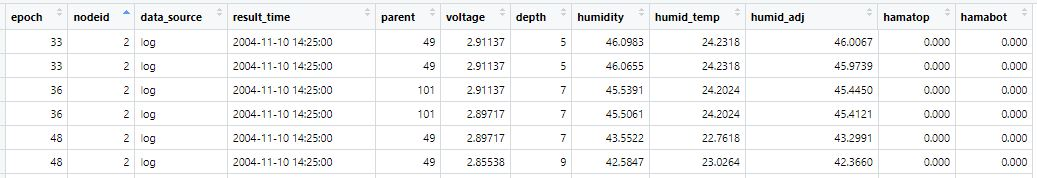
\includegraphics{./images/dupe_row.JPG}

\includegraphics{Red-Wood-Report_files/figure-latex/dupe-rows-by-nodeid-1.pdf}

\hypertarget{b---remove-missing-data}{%
\subsubsection{(b - remove missing
data)}\label{b---remove-missing-data}}

Duplicates and entries with readings greater than 3V or lower than 2.4V
were removed following procedure outlined in Tolle et al.. Table XX list
the record count after each removal step.

\begin{longtable}[]{@{}ll@{}}
\toprule
Data Removal Step & Record Count \\
\midrule
\endhead
Ingestion & 416,036 \\
Duplicate Removal & 393,213 \\
Voltage Removal & 264,144 \\
\bottomrule
\end{longtable}

\hypertarget{comment-on-the-number-of-missing-measurements-and-the-corresponding-datetime-period}{%
\subsubsection{Comment on the number of missing measurements and the
corresponding date/time
period?}\label{comment-on-the-number-of-missing-measurements-and-the-corresponding-datetime-period}}

There are 7568 row of readings containing at least a missing
measurement. The missing measurements have corresponding date between
May 25 to May 29 and at Nov 10.During May 25 to May 29, missing
measurements occurred throughout the day. Less errors occurred at noon
while more errors occurred at night and in the early morning. In Nov 10,
most error occurred at 14:25:00.

\hypertarget{c---incorporate-location-data-from-other-file}{%
\subsubsection{(c - incorporate location data from other
file)}\label{c---incorporate-location-data-from-other-file}}

After we joined the location data, we have 15 variables.

\hypertarget{d---visually-identify-outliers-for-each-of-following-humidity-humid-temp-hamatop-hamabot.-remove-and-comment-on-rationale-for-removing}{%
\subsubsection{(d - visually identify outliers for each of following:
humidity, humid temp, hamatop, hamabot. Remove and comment on rationale
for
removing)}\label{d---visually-identify-outliers-for-each-of-following-humidity-humid-temp-hamatop-hamabot.-remove-and-comment-on-rationale-for-removing}}

We can remove all humidity reading \textless{} 21 which is less than the
1\% quantile, humid\_temp \textgreater{} 100 which is larger than the
99\% quantile, maybe hamabot \textgreater{} 4000, which is larger than
the 98\% quantile.

\hypertarget{e-bonus---discuss-other-possible-outliers-and-explain-reason-why-it-is-better-to-remove-them-than-to-keep}{%
\subsubsection{(e bonus - discuss other possible outliers and explain
reason why it is better to remove them than to
keep)}\label{e-bonus---discuss-other-possible-outliers-and-explain-reason-why-it-is-better-to-remove-them-than-to-keep}}

\begin{center}\rule{0.5\linewidth}{0.5pt}\end{center}

\hypertarget{data-exploration}{%
\subsection{3 Data Exploration}\label{data-exploration}}

\hypertarget{a-dylan}{%
\subsubsection{(a) (Dylan)}\label{a-dylan}}

\hypertarget{b-dylan}{%
\subsubsection{(b) (Dylan)}\label{b-dylan}}

\hypertarget{c-dylan}{%
\subsubsection{(c) (Dylan)}\label{c-dylan}}

\hypertarget{d-dylan}{%
\subsubsection{(d) (Dylan)}\label{d-dylan}}

\begin{center}\rule{0.5\linewidth}{0.5pt}\end{center}

Idea List (things to investigate): - is a tree sentient? Does the
weather from the previous n days affect any of the measurement readings
collected? For example, would a series of dry days show any humidity
differences in or around the tree? - Influence points. How much can the
distributions be shifted by missing values (mentioned in article as
future work). Does the missing data affect any of the findings? - How
does the collected data match up with any weather trends in the area?
Maybe the tree had higher humidity rates for example than normal ground.

\hypertarget{a-andrew}{%
\subsubsection{(a) (Andrew)}\label{a-andrew}}

\hypertarget{b-andrew}{%
\subsubsection{(b) (Andrew)}\label{b-andrew}}

\hypertarget{c-andrew}{%
\subsubsection{(c) (Andrew)}\label{c-andrew}}

\hypertarget{d-andrew}{%
\subsubsection{(d) (Andrew)}\label{d-andrew}}

\begin{center}\rule{0.5\linewidth}{0.5pt}\end{center}

\hypertarget{interesting-findings}{%
\subsection{4 Interesting Findings}\label{interesting-findings}}

\begin{center}\rule{0.5\linewidth}{0.5pt}\end{center}

\hypertarget{graph-critique-in-the-paper}{%
\subsection{5 Graph Critique in the
Paper}\label{graph-critique-in-the-paper}}

\hypertarget{log-transform-of-histograms}{%
\subsubsection{Log Transform of
Histograms}\label{log-transform-of-histograms}}

The incident and reflected PAR histograms from Tolle et al.~(figure 3a)
have long tails and with large numbers of observations around 0 which
make the charts hard to discern. We present this data after taking a log
transform of the observations and present the results side-by-side with
the initial chart versions (non-log scale).
\includegraphics{Red-Wood-Report_files/figure-latex/5a-incident-charts-1.pdf}
\includegraphics{Red-Wood-Report_files/figure-latex/5a-incident-charts-2.pdf}
Both log charts visually convey the long tail better than the non-log
counter-parts. In fact, the log scale displays a bimodal distributions
that could be interpreted as light levels during the day and at night.

however, some readers might be mislead/confused by the log
interpretation. At first glance, PAR measurements appear more
concentrated around a smaller range and it's important readers
understand the log function before reaching an incorrect conclusion
derived from the plots. We've displayed both versions for clarity.

\includegraphics{Red-Wood-Report_files/figure-latex/5a-reflected-charts-1.pdf}
\includegraphics{Red-Wood-Report_files/figure-latex/5a-reflected-charts-2.pdf}

\hypertarget{boxplot-analysis---daytime-measurements-only}{%
\subsubsection{Boxplot Analysis - Daytime Measurements
Only}\label{boxplot-analysis---daytime-measurements-only}}

\begin{figure}
\centering
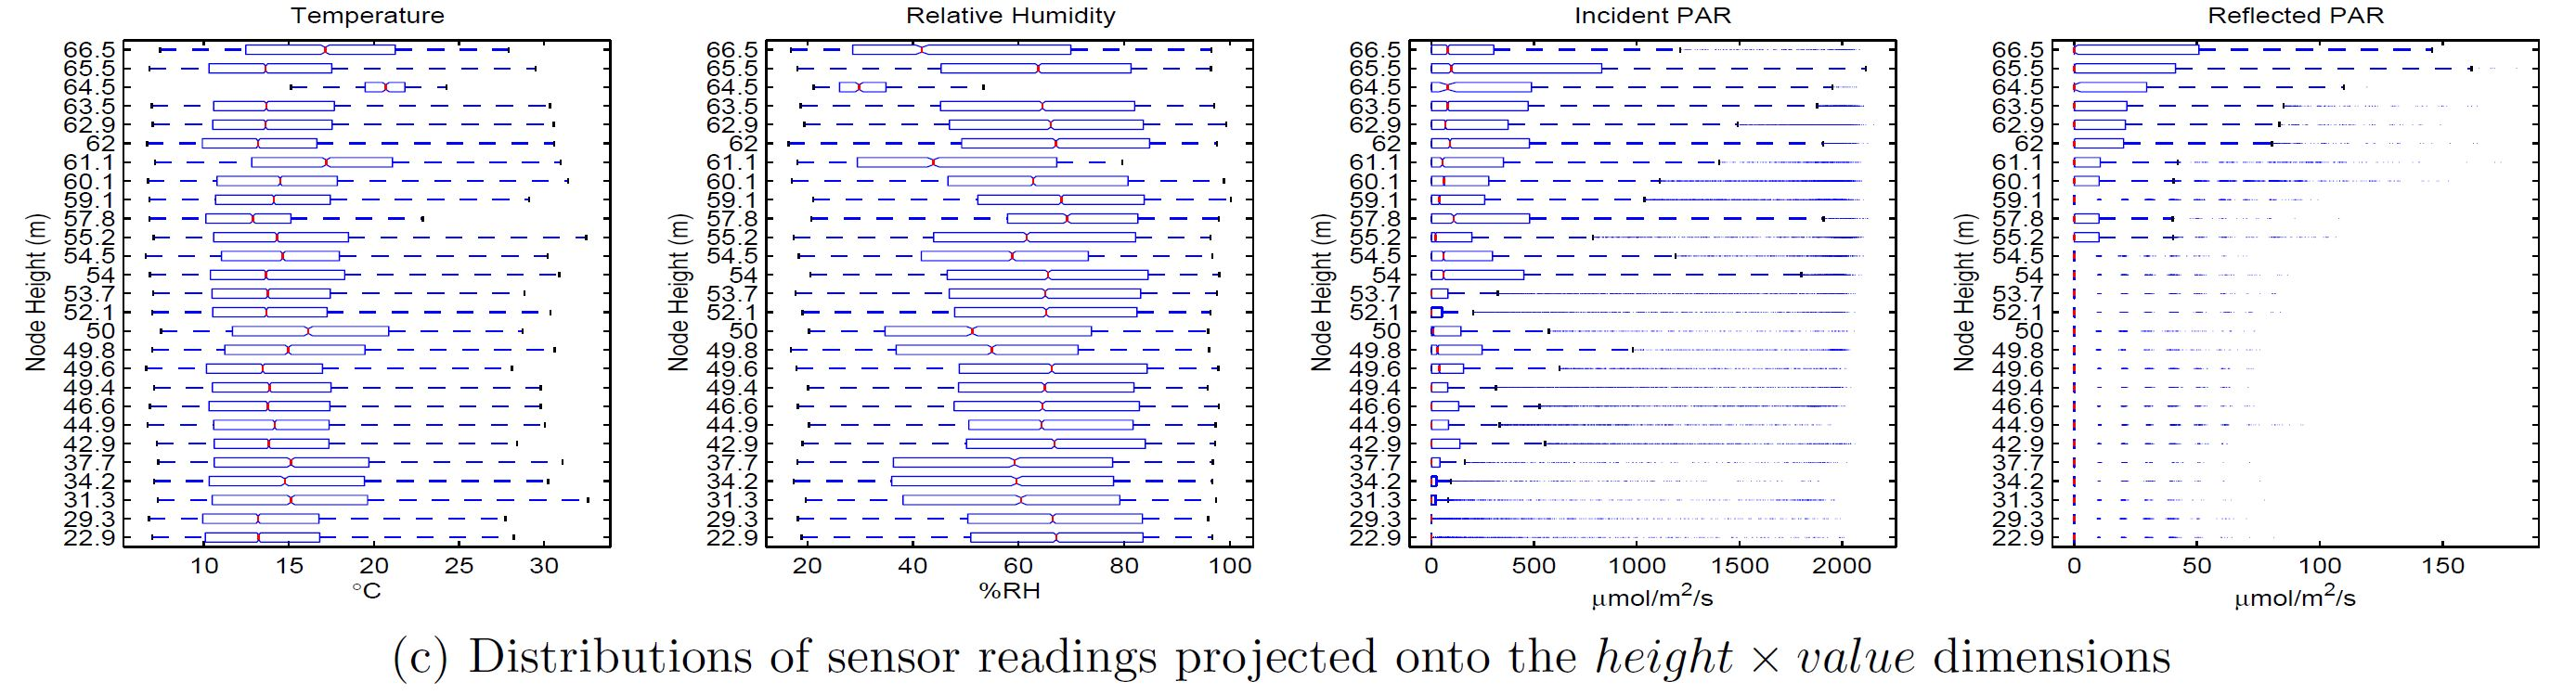
\includegraphics{./images/3c_plot_pic.JPG}
\caption{Original Tolle Boxplots - 3c}
\end{figure}

The boxplots from Figure 3{[}c{]} in the orginal paper are showing how
the sensor measurements vary over the height of the tree. Tolle et
al.~are attempting to look for spatial gradients and trends by
eliminating the temporal aspect of the data.

With regards to the PAR charts I don't believe these plots convey the
right message. I think the author should have split up the temporal
ranges included in this chart. For example, the PAR temporal range
should only include daytime, when the sun is shining. Including the full
temporal range adds a large number of data points with 0 light readings
and effectively pulls the mass closer to zero for all readings and makes
the gradient less pronounced.

We plotted the charts only considering daylight hours.

\includegraphics{Red-Wood-Report_files/figure-latex/q5b-height-value-box-plots-1.pdf}

Some statement here about how the gradients over height become more
clear when we strip out the night time measurements.

\begin{figure}
\centering
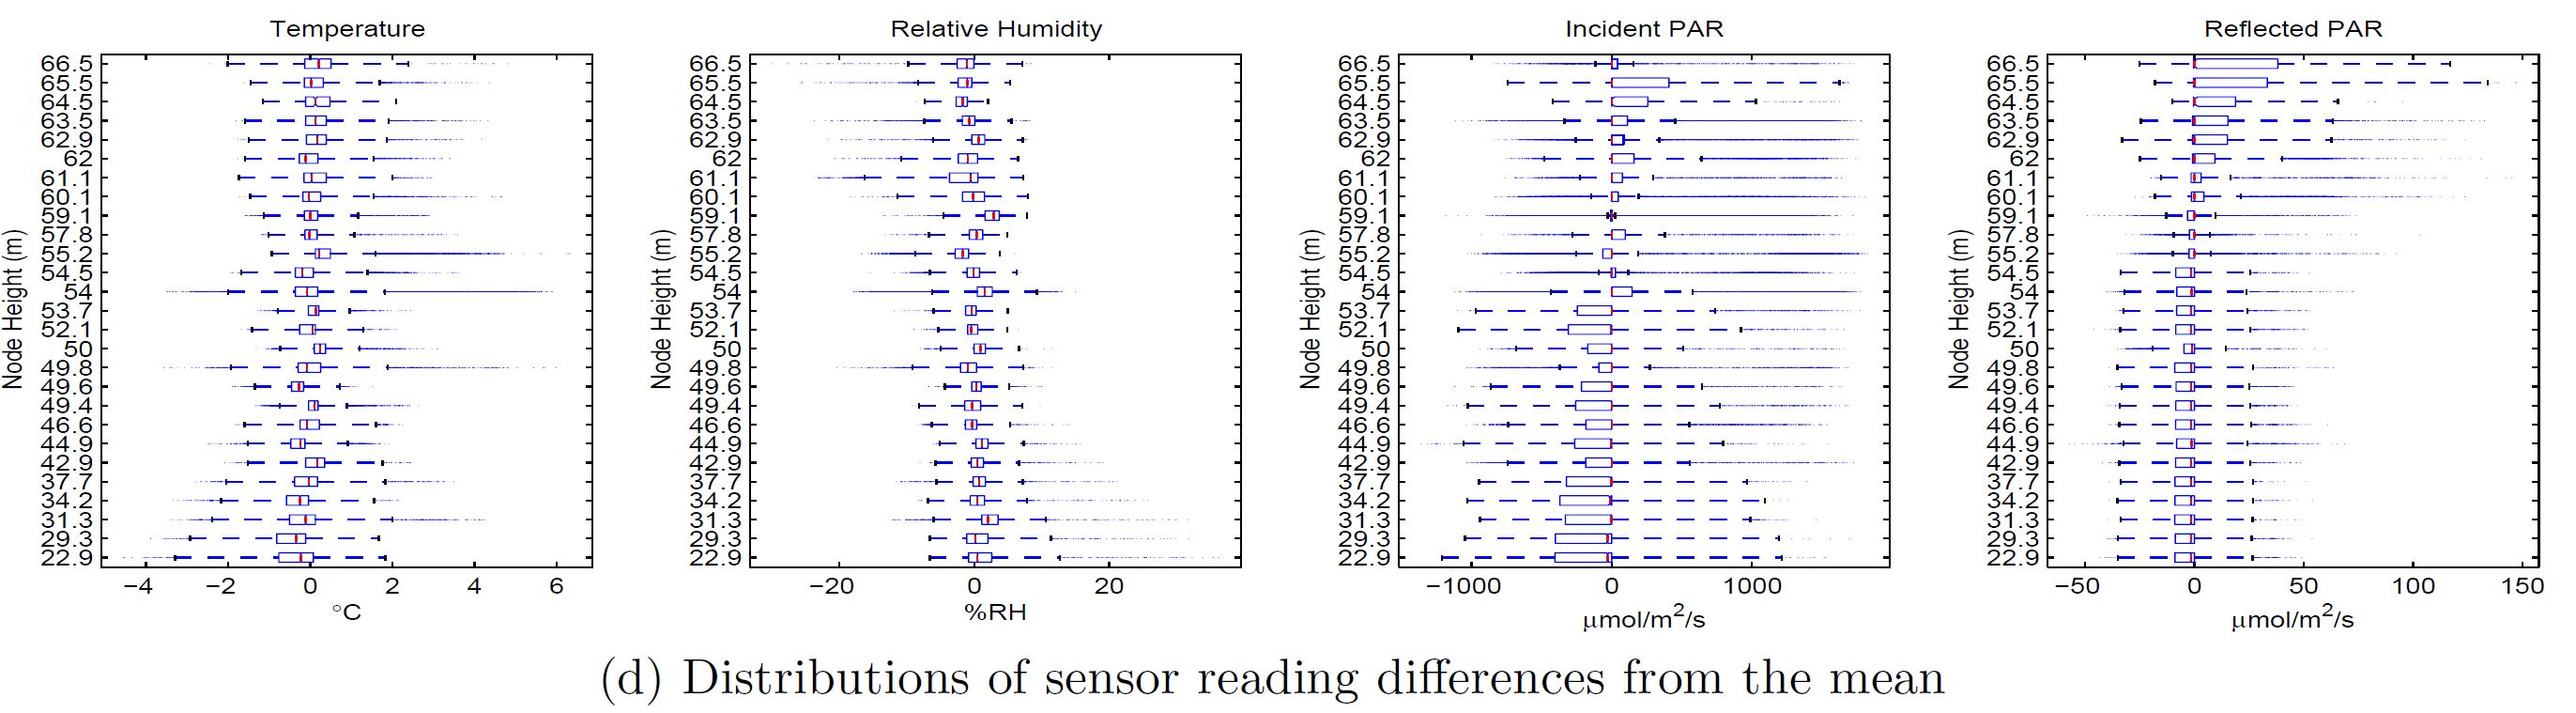
\includegraphics{./images/3d_plot_pic.JPG}
\caption{Original Tolle Boxplots - 3d}
\end{figure}

\hypertarget{tolle-figure-4-plot-suggestions}{%
\subsubsection{Tolle Figure 4 Plot
Suggestions}\label{tolle-figure-4-plot-suggestions}}

Any suggestions for improving the first two plots in Figure 4? Can you
distinguish all the colors in these two plots?

I think discretizing the time plot (maybe showing every hour) would make
the content more digestiable. Both charts are also lacking a legend and
leave the onus on the reader to discern which heights correspond to
which colors. To more clearly show height gradient we believe using a
two-color continuum (shortest to tallest) would more clearly display the
trend similar to what the author did in Figure 5.

\hypertarget{tolle-figure-7-comment}{%
\subsubsection{Tolle Figure 7 Comment}\label{tolle-figure-7-comment}}

Comment on Figure 7. Is it possible to generate a better visualization
to highlight the difference between network and log data?

We believe that overlaying the bar charts might create better contrast
between the two sources.

\hypertarget{appendix}{%
\subsection{Appendix}\label{appendix}}

Extra Charts:

Duplicate record chart

Histogram plots of all variables

\end{document}
